
% This LaTeX was auto-generated from MATLAB code.
% To make changes, update the MATLAB code and republish this document.

\documentclass{article}
\usepackage{graphicx}
\usepackage{color}

\sloppy
\definecolor{lightgray}{gray}{0.5}
\setlength{\parindent}{0pt}

\begin{document}

    
    \begin{verbatim}
clear; close all;clc;
\end{verbatim}

\begin{verbatim}Measuring transfer functions\end{verbatim}
    \begin{verbatim}
% Generation of multisine signals.

t = 1:4096;     % Time
K_max = 100;
K = 1:K_max;      % Number of excited spectral lines

% Constant phase multisine
phi = 0;
multisine = sum(sin(2*pi*t'*K/length(t) + phi),2);

% Random phase mutlisine
phi = 2*pi*rand([1,K_max]);
multisine_rand = sum(sin(2*pi*t'*K/length(t) + phi),2);

% Schroeder phase
phi = K.*(K+1)*pi/length(K);
multisine_schro = sum(sin(2*pi*t'*K/length(t) + phi),2);

% Crest factor

% Crest factor - constant phase multisine
crestFact = max(multisine)/rms(multisine);

% Crest factor - random phase mutlisine
crestFact_rand = max(multisine_rand)/rms(multisine_rand);

% Crest factor - Schroeder phase mutlisine
crestFact_schro = max(multisine_schro)/rms(multisine_schro);

disp('Crest factors: ');
disp(join(['Constant phase multisine:  ',num2str(crestFact)]));
disp(join(['Random phase multisine:    ',num2str(crestFact_rand)]));
disp(join(['Schroeder phase multisine: ',num2str(crestFact_schro)]));

% FFTs

% FFT - constant phase multisine
fft_const = fftshift(fft(multisine));

% FFT - random phase multisine
fft_rand = fftshift(fft(multisine_rand));

% FFT - Schroeder phase multisine
fft_schro = fftshift(fft(multisine_schro));

% Plots
fq = -length(t)/2:length(t)/2 -1;

figure('Position',[500 500 800 420]);hold on;
subplot(1,2,1)
plot(t',multisine',t',multisine_rand,t',multisine_schro);
legend('Constant phase spectrum','random phase spectrum','Schroeder phase spectrum');

subplot(1,2,2)
plot(fq,abs(fft_const),fq,abs(fft_rand),fq,abs(fft_schro));
xlim([-300 300]);
legend('Constant phase spectrum','random phase spectrum','Schroeder phase spectrum');

figure;hold on;
subplot(3,2,1);
plot(t',multisine');
xlabel('Time samples');

subplot(3,2,3);
plot(t',multisine_rand');
xlabel('Time samples');

subplot(3,2,5);
plot(t',multisine_schro');
xlabel('Time samples');

subplot(3,2,2);
plot(fq,abs(fft_const));
xlabel('Frequency');

subplot(3,2,4);
plot(fq,abs(fft_rand));
xlabel('Frequency');

subplot(3,2,6);
plot(fq,abs(fft_schro));
xlabel('Frequency');
\end{verbatim}

        \color{lightgray} \begin{verbatim}Crest factors: 
Constant phase multisine:  10.2979
Random phase multisine:    3.5714
Schroeder phase multisine: 1.908
\end{verbatim} \color{black}
    
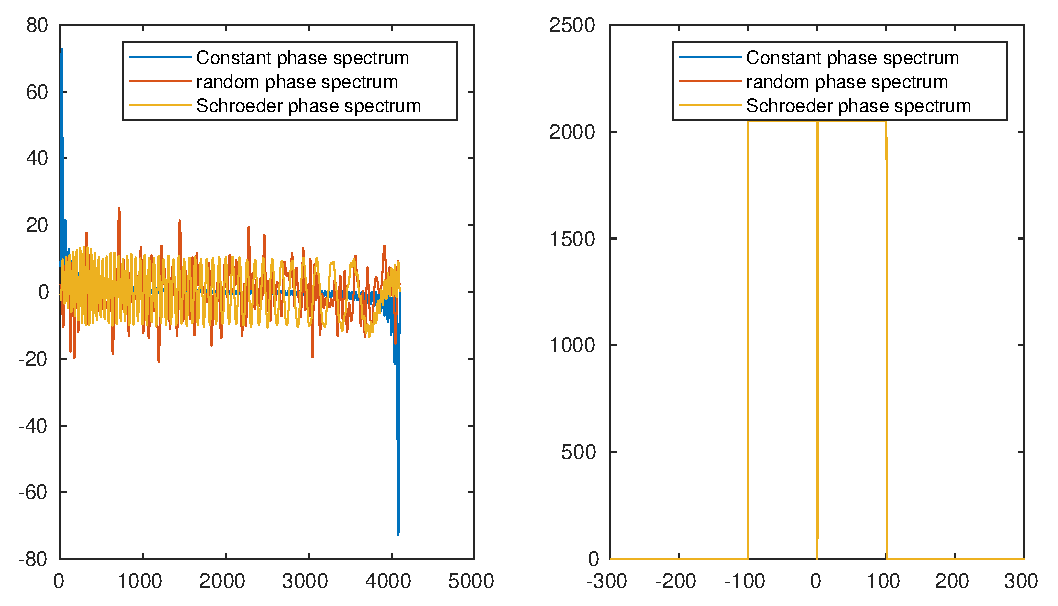
\includegraphics [width=4in]{main_01.eps}

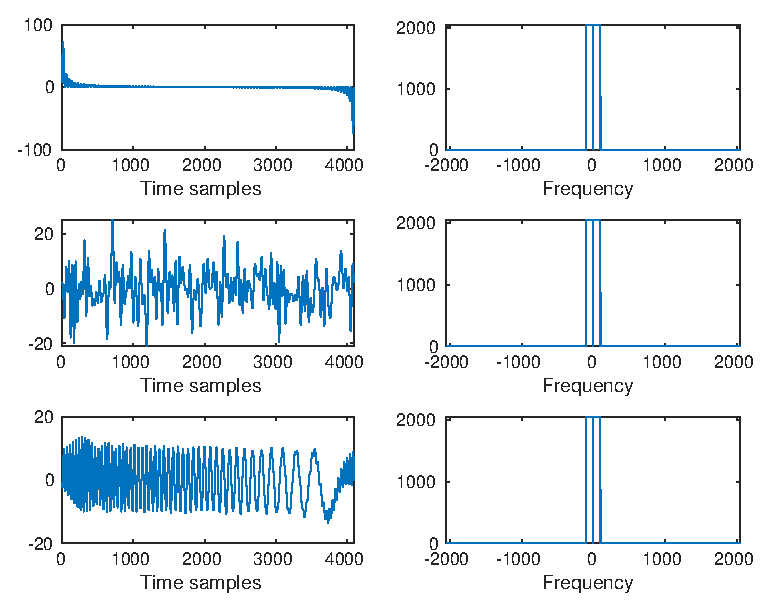
\includegraphics [width=4in]{main_02.eps}
\begin{par}
DUT measurements
\end{par} \vspace{1em}
\begin{verbatim}
% DUT parameters

bandwidth = 500;
fs = 8e3;          % Sampling frequency

% Generation of the multisine
\end{verbatim}
\begin{par}
$\omega_{0} = \frac{2\pi f_{s}}{N}$
\end{par} \vspace{1em}
\begin{verbatim}
N = fs;
t = 1:N;
K_max = 500;
K = 1:K_max;      % Number of excited spectral lines

% Schroeder phase
phi = K.*(K+1)*pi/length(K);
u_sch_500 = sum(sin(2*pi*t'*K/length(t) + phi),2);
u_sch_500 = 0.1*u_sch_500/rms(u_sch_500);

% FFT
fft_u_sch_500 = fftshift(fft(u_sch_500));

% Plots
figure('Position',[500 500 800 420]);hold on;
subplot(1,2,1)
plot(t',u_sch_500);
legend('Schroeder phase spectrum');

fq = -length(t)/2:length(t)/2 -1;
subplot(1,2,2)
plot(fq,abs(fft_u_sch_500));
xlim([-700 700]);
legend('Schroeder phase spectrum');

% Save the input signal
save('Group9_Input1.mat','u_sch_500');
\end{verbatim}

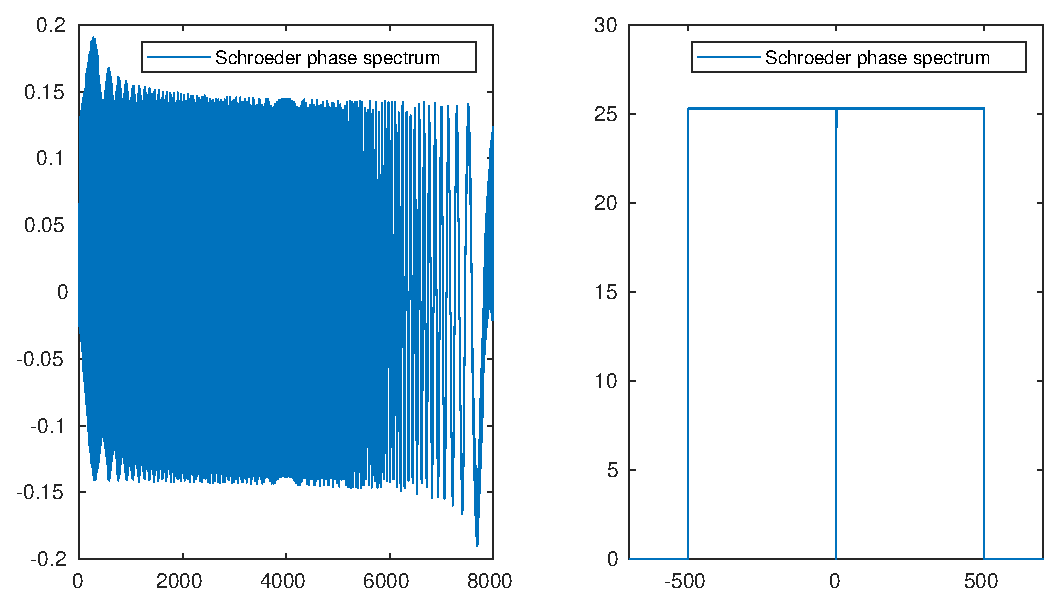
\includegraphics [width=4in]{main_03.eps}
\begin{par}
Excitation signals
\end{par} \vspace{1em}
\begin{verbatim}
% Periodic

% Constant phase multisine
phi = 2*pi*0;
multisine_const = sum(sin(2*pi*t'*K/length(t) + phi),2);
multisine_const = 0.1*multisine_const/rms(multisine_const);

% Random phase mutlisine
phi = 2*pi*rand([1,K_max]);
multisine_rand = sum(sin(2*pi*t'*K/length(t) + phi),2);
multisine_rand = 0.1*multisine_const/rms(multisine_rand);

% Periodic noise signal
d = 1;
period = N/d;
noise_per = randn([period,1]);
noise_per = repmat(noise_per,d);
noise_per = 0.1*noise_per/rms(noise_per);

% Aperiodic

noise_aper = randn([N,1]);
noise_aper = 0.1*noise_aper/rms(noise_per);

% Multiplyin the noise by the Hanning window
[Hann] = hanning(N,'periodic');
noise_aper_h = noise_aper.*Hann;

figure('Position',[500 500 800 420]);hold on;
subplot(1,2,1);
plot(noise_aper);
subplot(1,2,2);
plot(t,noise_aper_h,t,Hann);
\end{verbatim}

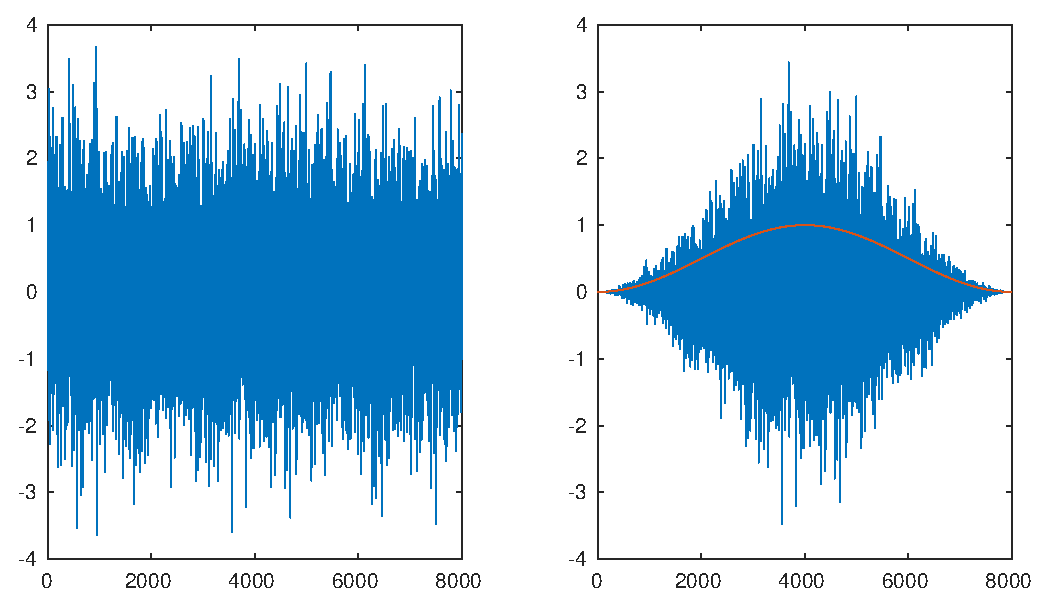
\includegraphics [width=4in]{main_04.eps}



\end{document}
    
